\section{Cross-model OCEAN transfer matrices}\label{sec:appendix-crossmodel-matrices}

The main supervised results (\Cref{sec:supervised}) were produced on
Llama-3.1-8B-Instruct. To test how the persona-LoRA recipe behaves across base
models, we re-ran the full paired-DPO pipeline (\Cref{sec:training-loras}) ---
holding the constitution, distillation procedure, and training hyper-parameters
fixed --- on six base models spanning three families and a $4\times$ size range:
Llama-3.1-8B-Instruct \citep{grattafiori2024llama}, Qwen3-8B and Qwen3-32B
\citep{qwen2025qwen3}, and Gemma-3 4B/12B/27B-IT \citep{gemma_2025}. This yields
the full set of $5$ traits $\times$ $\{$amplifier, suppressor$\}$ adapters plus a
null control adapter for every model.

\paragraph{What the matrices show.} For each base model and each applied OCEAN
adapter we sweep the LoRA scalar and, at every scale, measure the
\texttt{TRAIT}-logprob MCQ score (\Cref{sec:appendix-e}) for \emph{all five}
OCEAN traits. \Cref{fig:crossmodel-trait-amp,fig:crossmodel-trait-sup} arrange
this as a $5\times 5$ matrix: columns index the applied adapter, rows index the
measured trait, and each cell is a LoRA-scale sweep with one line per base
model. The bold-bordered cells on the diagonal are the on-target panels (measured
trait $=$ applied trait); off-diagonal cells show cross-trait leakage. Colour
encodes family (Llama blue, Qwen orange/red, Gemma green) and darkens with model
size; each model has its own marker.

\paragraph{Reading the trends.} The recipe transfers across families and sizes:
on every diagonal the target trait moves in the intended direction at the trained
scale and returns to baseline near scale $0$, for all six models. Off-diagonal
movement is comparatively small in the working range ($|c|\lesssim 2$), i.e.\ the
adapters are reasonably trait-specific, though some structured leakage is visible
(e.g.\ between conscientiousness and neuroticism). The null control adapter
(\Cref{fig:crossmodel-trait-control}) stays approximately flat across all five
traits, confirming that the paired-DPO procedure itself induces little spurious
trait shift.

\paragraph{Method notes.} Per-sample scores are filtered to answers with choice
mass $\geq 0.75$ (matching the eval's own metric), and a sweep point is dropped
when fewer than $10$ samples survive that filter --- otherwise a near-degenerate
generation at an extreme scale would yield a meaningless interval. Trait error
bars are $95\%$ bootstrap CIs; MMLU error bars
(\Cref{fig:crossmodel-mmlu,fig:crossmodel-mmlu-control}) are Wilson intervals.

\begin{figure}[p]
\centering
% Generated by: scripts/visualisations/model_comparison_ocean_transfer.py
% Data: HF persona-shattering-lasr/monorepo @ fine_tuning/{model}/ocean/{trait}/{dir}/{ver}/evals/mcq/trait_logprobs/ for the 6 base models — see paper/figures/MANIFEST.md
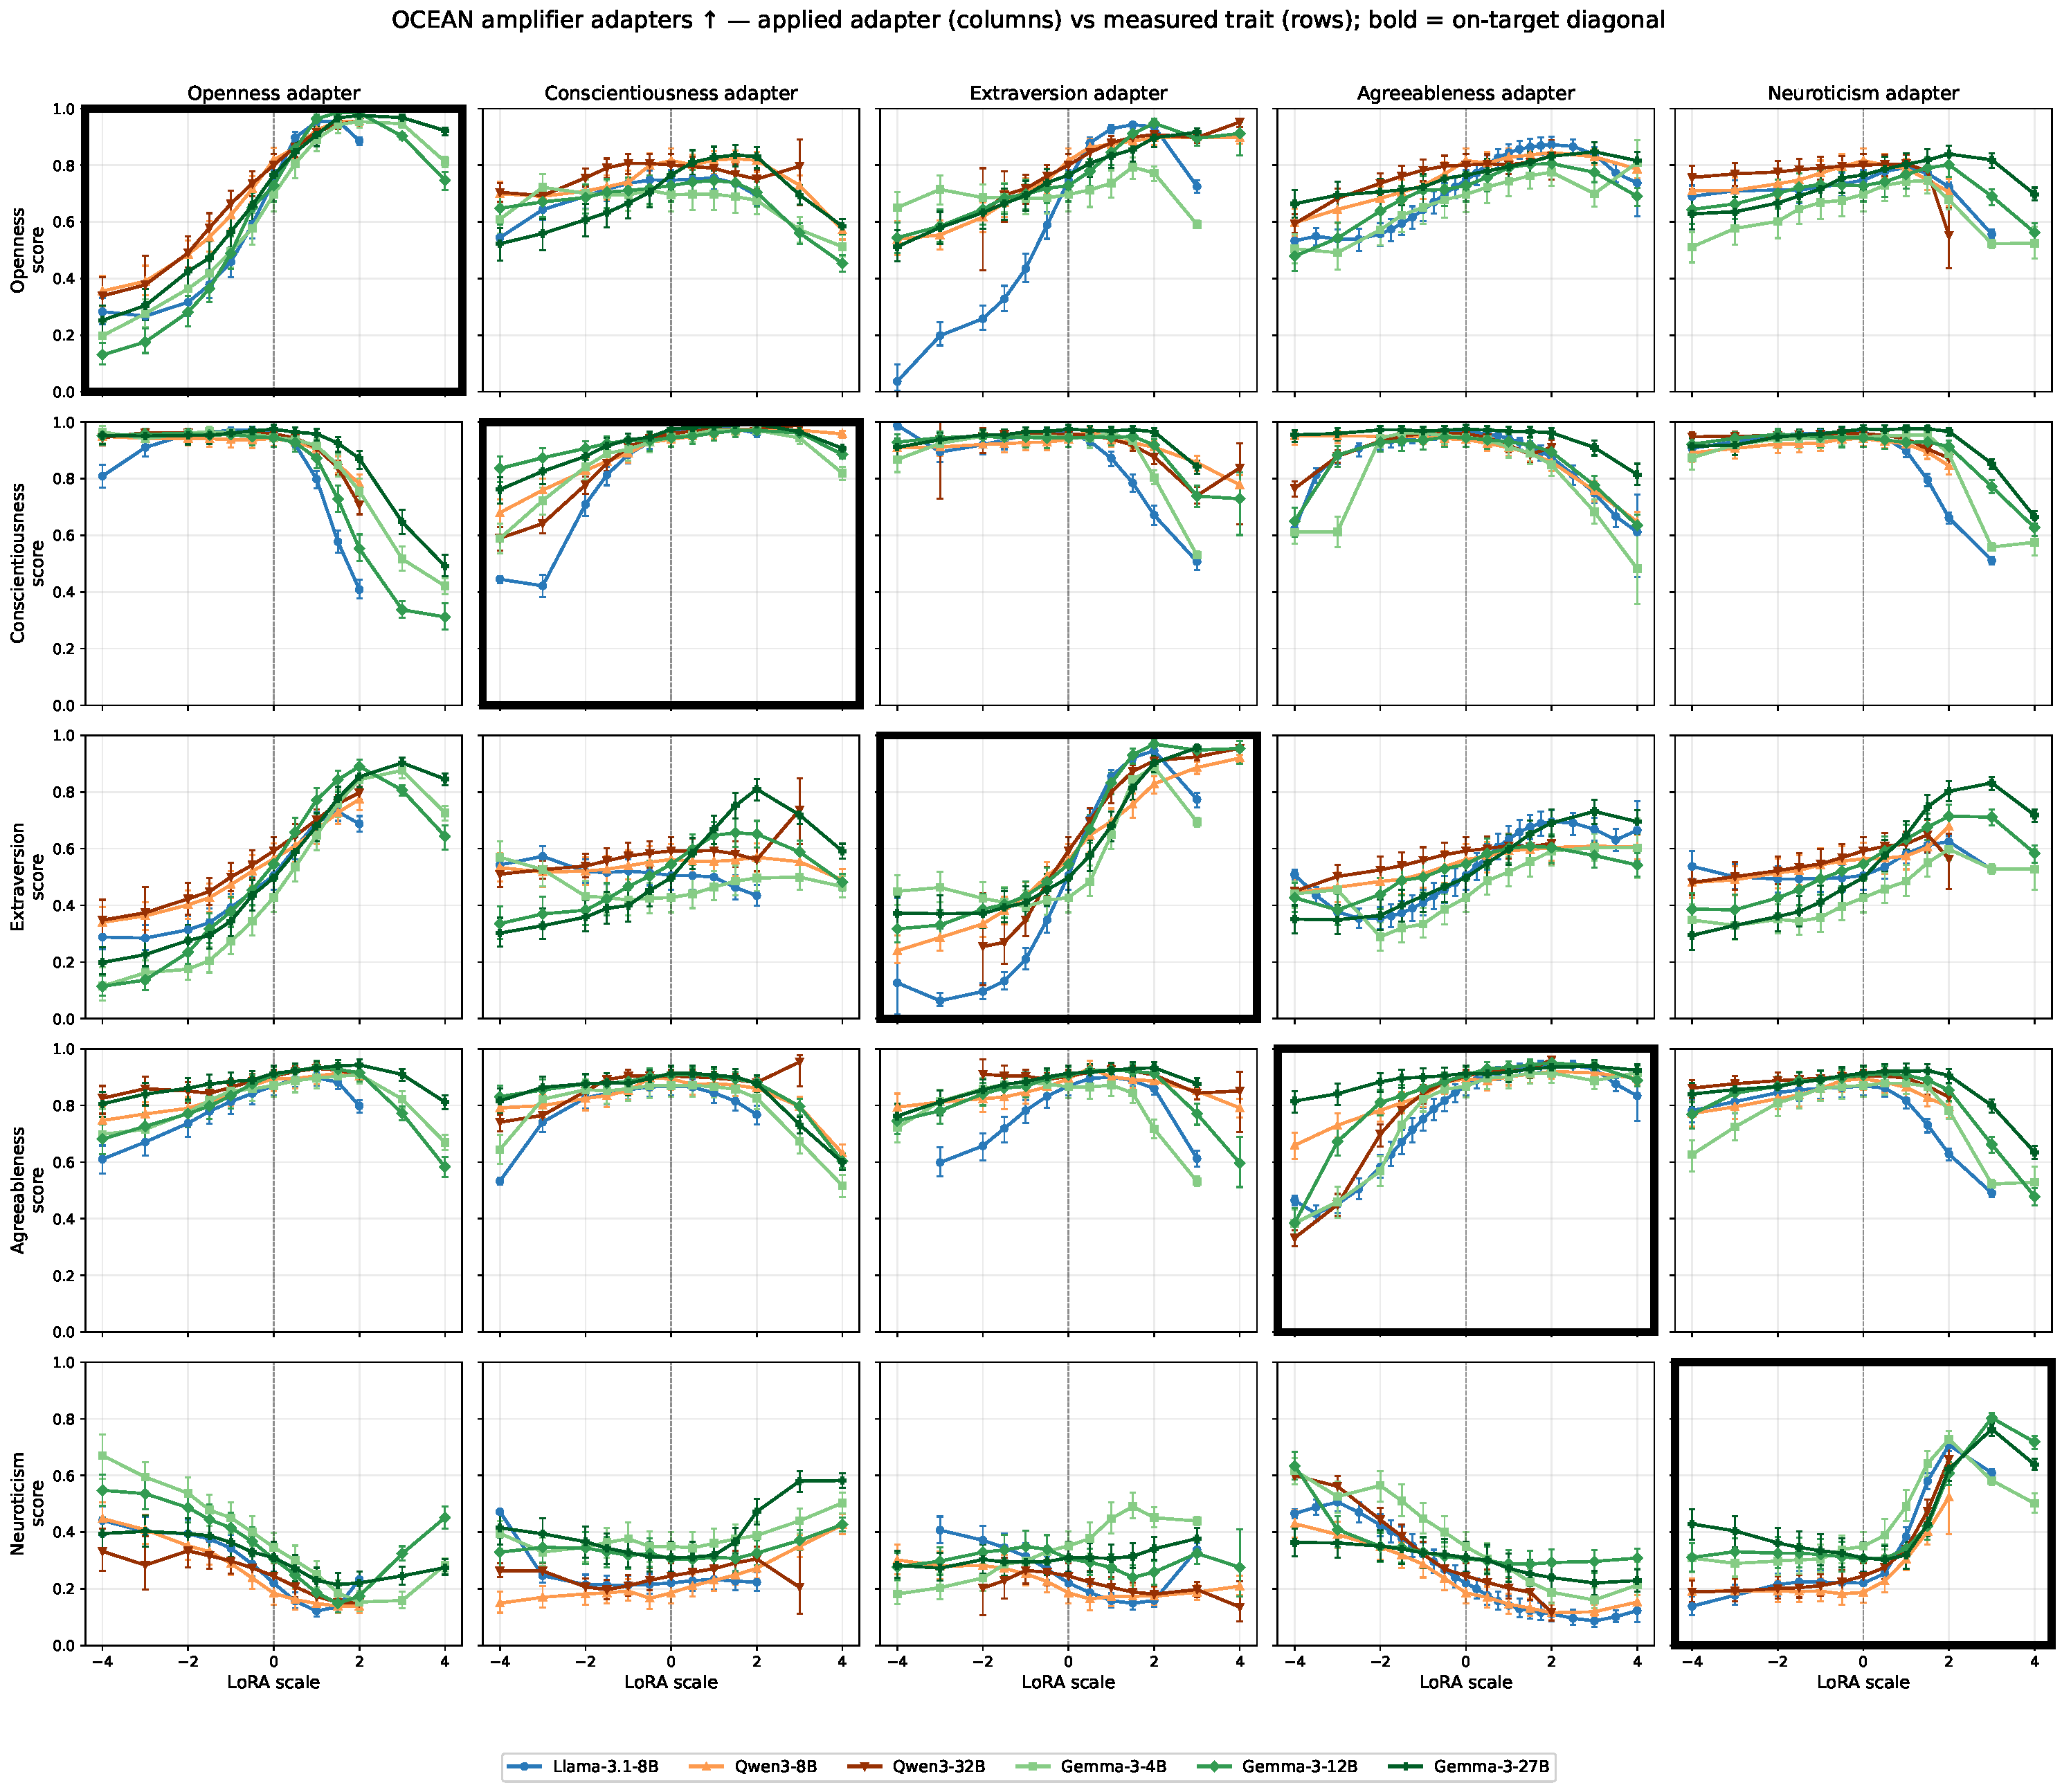
\includegraphics[width=\linewidth]{figures/appendix/model_comparison/fig_crossmodel_trait_amplifier.pdf}
\caption{\textbf{Amplifier transfer matrix across base models.} Columns: applied
OCEAN \emph{amplifier} adapter; rows: measured OCEAN trait
(\texttt{TRAIT}-logprob MCQ score, $0$--$1$) vs LoRA scale. One line per base
model. Bold-bordered diagonal panels are on-target (measured $=$ applied).}
\label{fig:crossmodel-trait-amp}
\end{figure}

\begin{figure}[p]
\centering
% Generated by: scripts/visualisations/model_comparison_ocean_transfer.py
% Data: HF persona-shattering-lasr/monorepo @ fine_tuning/{model}/ocean/{trait}/{dir}/{ver}/evals/mcq/trait_logprobs/ for the 6 base models — see paper/figures/MANIFEST.md
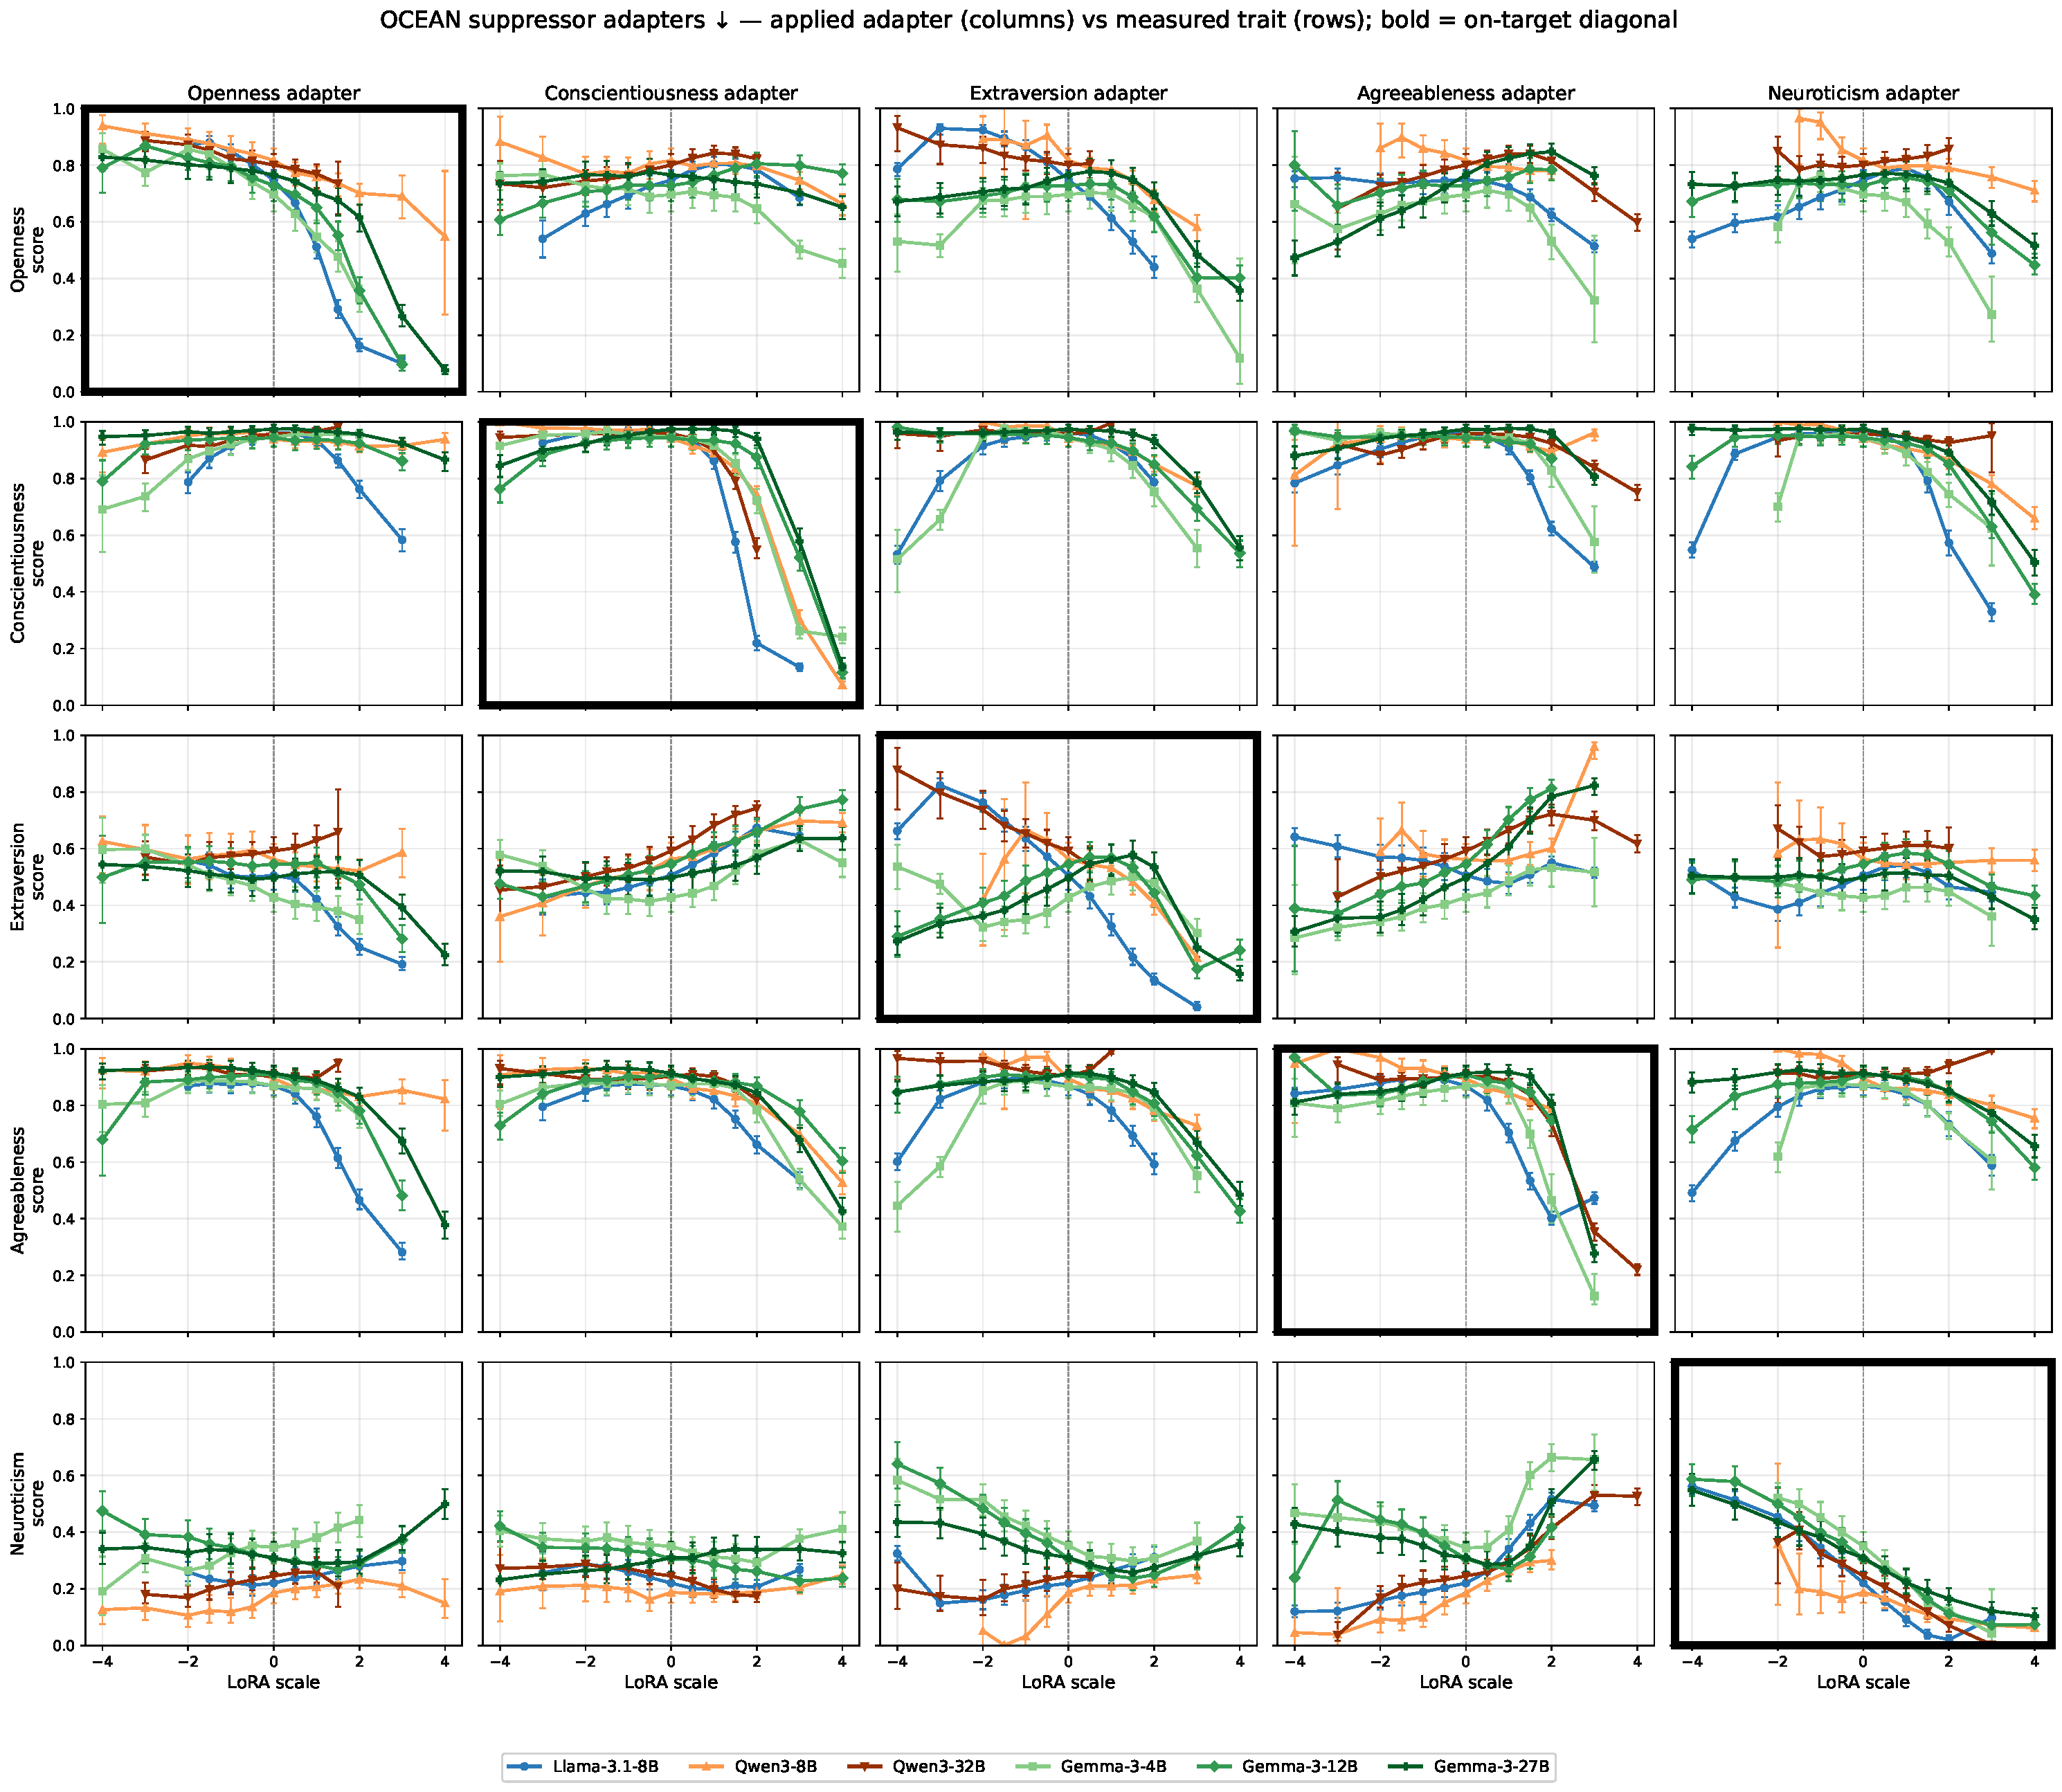
\includegraphics[width=\linewidth]{figures/appendix/model_comparison/fig_crossmodel_trait_suppressor.pdf}
\caption{\textbf{Suppressor transfer matrix across base models.} As
\Cref{fig:crossmodel-trait-amp} but for the \emph{suppressor} adapters: the
on-target diagonal moves the measured trait downward in the intended direction.}
\label{fig:crossmodel-trait-sup}
\end{figure}

\begin{figure}[htbp]
\centering
% Generated by: scripts/visualisations/model_comparison_ocean_transfer.py
% Data: HF persona-shattering-lasr/monorepo @ fine_tuning/{model}/other/ocean_def_control/amplifier/{ver}_s1vs2/evals/mcq/trait_logprobs/ for the 6 base models — see paper/figures/MANIFEST.md
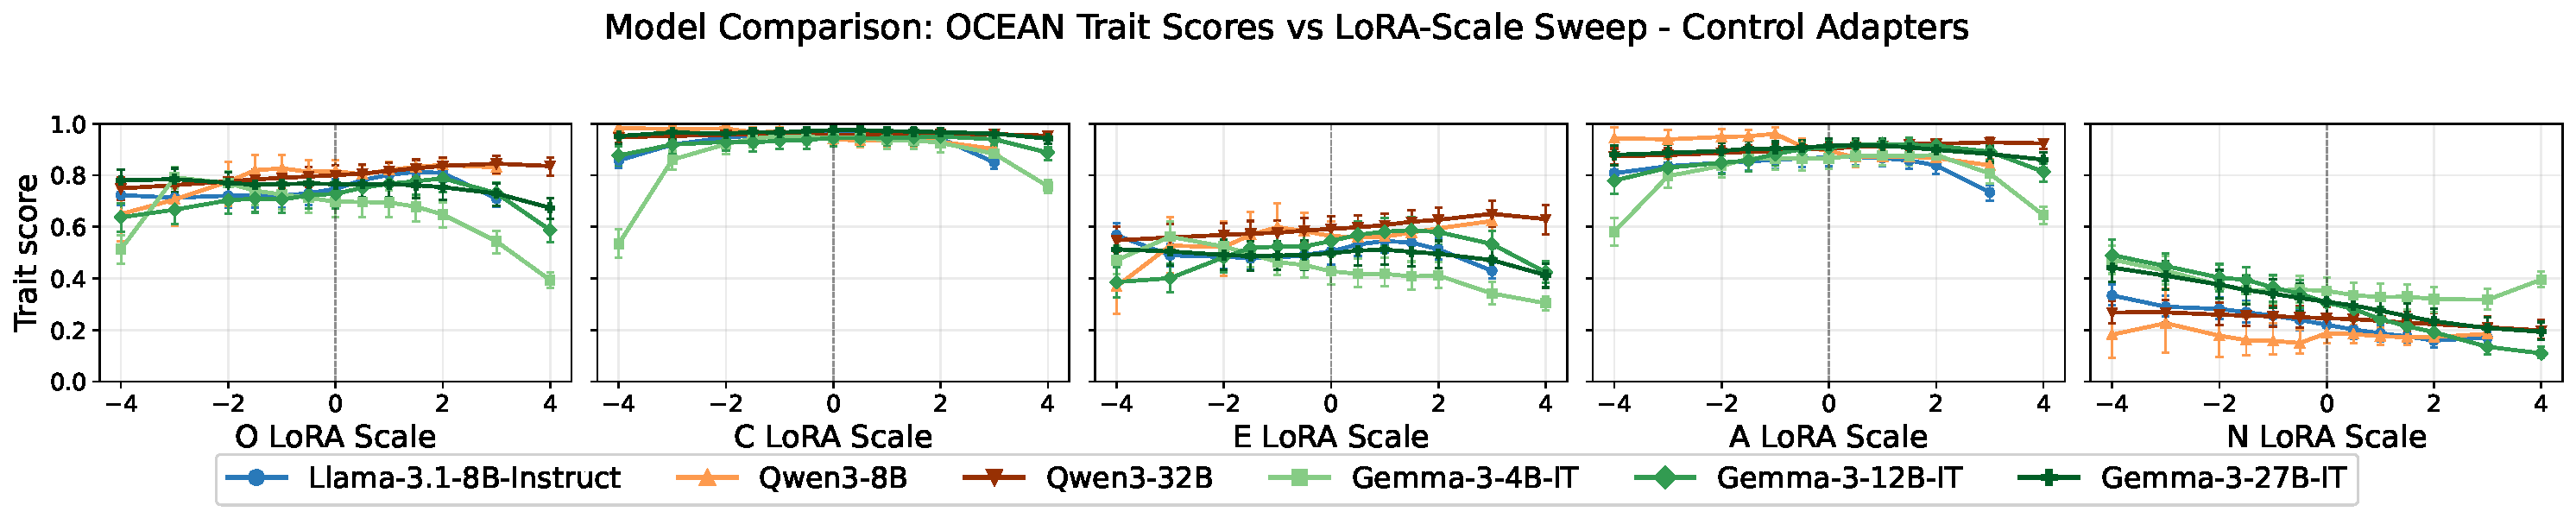
\includegraphics[width=\linewidth]{figures/appendix/model_comparison/fig_crossmodel_trait_control.pdf}
\caption{\textbf{Null control adapter across base models.} The seed-1-vs-seed-2
paired-DPO control adapter, with no trait constitution, measured on each of the
five OCEAN traits vs LoRA scale. Approximately flat curves indicate the training
procedure itself does not induce spurious trait shift.}
\label{fig:crossmodel-trait-control}
\end{figure}

\begin{figure}[htbp]
\centering
% Generated by: scripts/visualisations/model_comparison_ocean_transfer.py
% Data: HF persona-shattering-lasr/monorepo @ fine_tuning/{model}/ocean/{trait}/{dir}/{ver}/evals/mcq/mmlu/ for the 6 base models — see paper/figures/MANIFEST.md
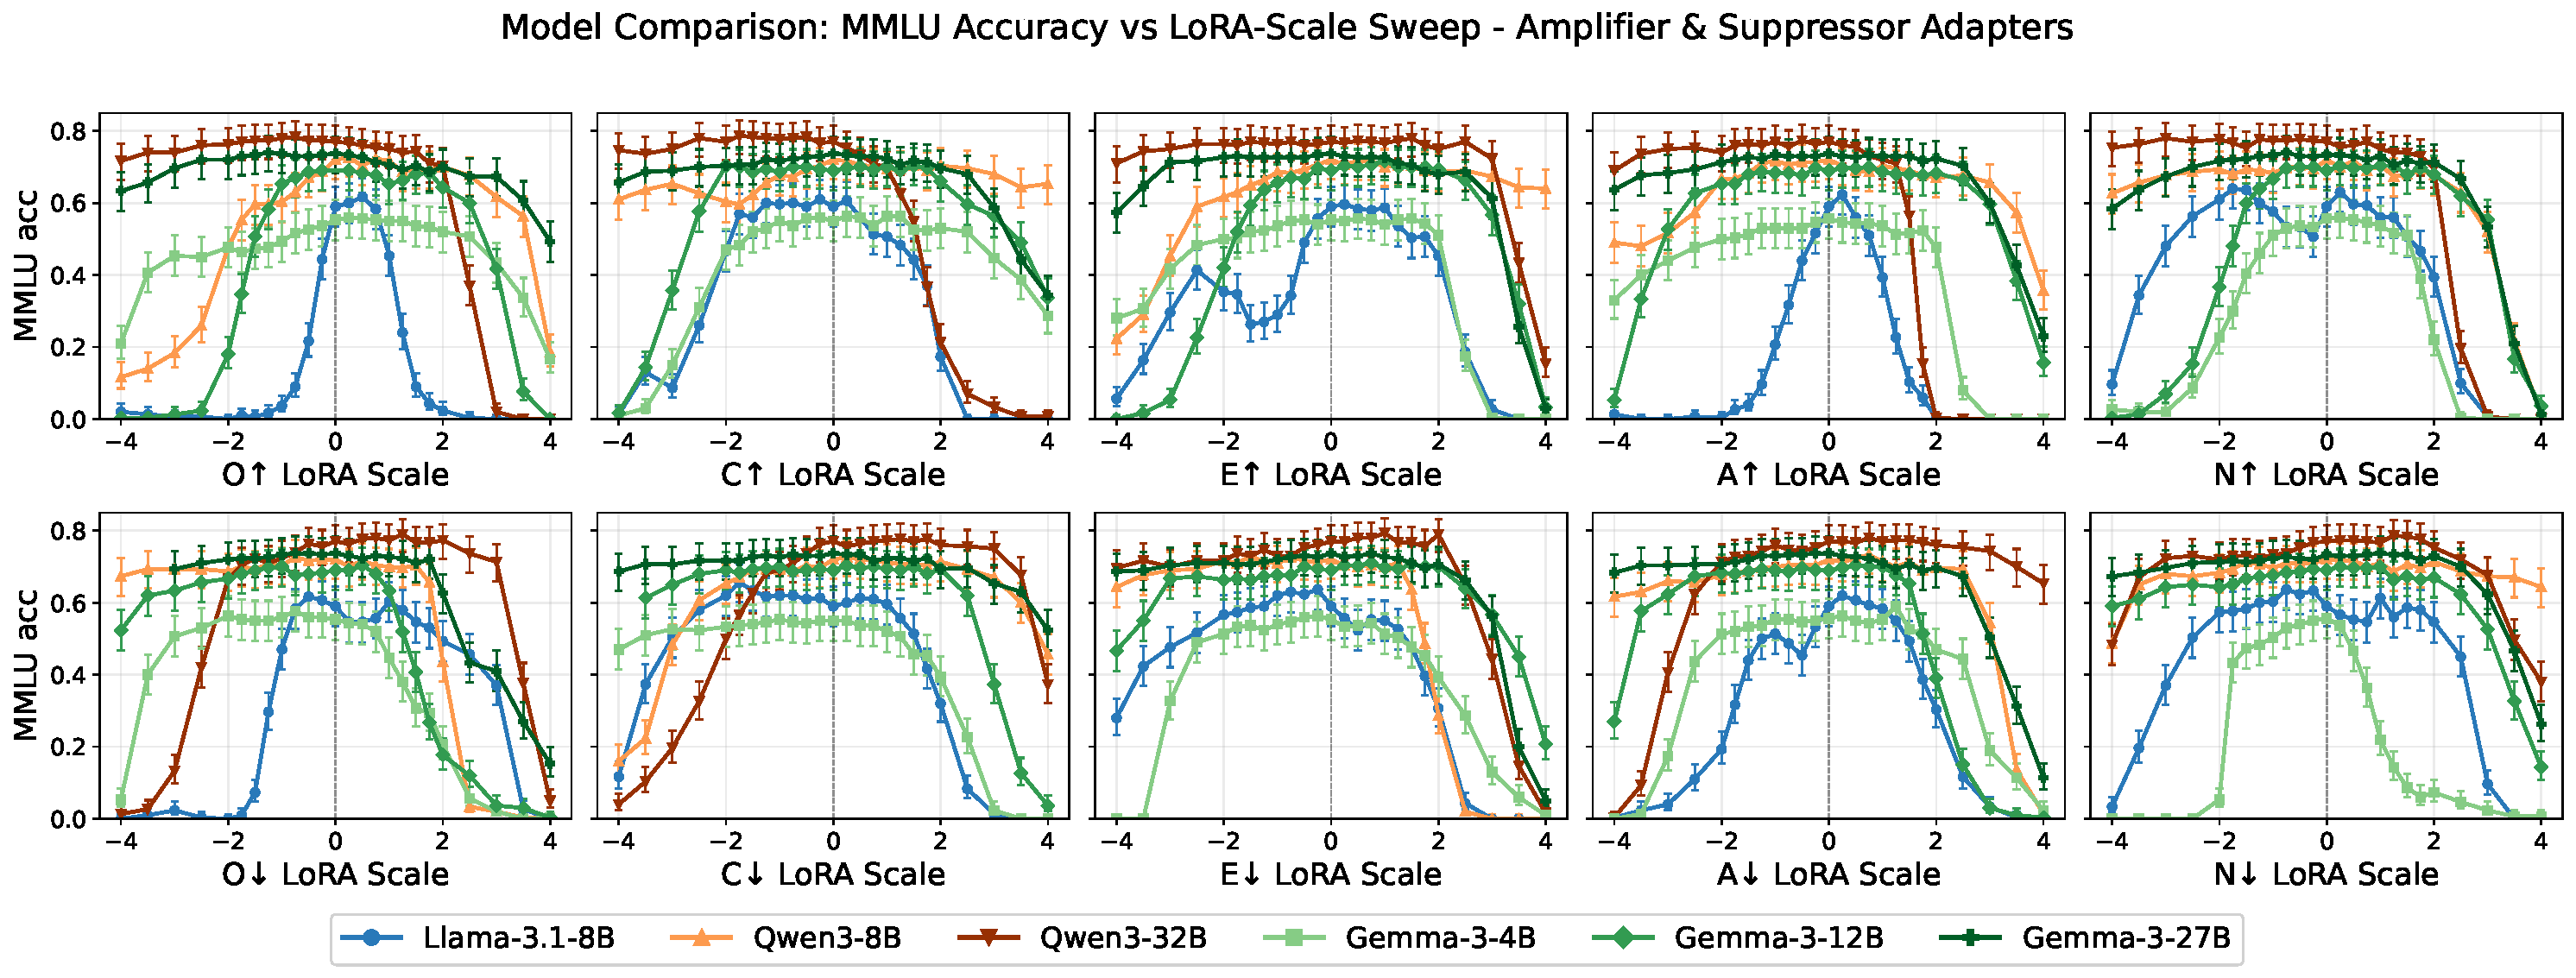
\includegraphics[width=\linewidth]{figures/appendix/model_comparison/fig_crossmodel_mmlu.pdf}
\caption{\textbf{MMLU capability retention across base models.} Rows: adapter
direction (amplifier / suppressor); columns: applied OCEAN adapter. MMLU
accuracy vs LoRA scale, one line per base model. Capability is largely preserved
in the working range and degrades at large $|c|$, more so for the smaller
checkpoints.}
\label{fig:crossmodel-mmlu}
\end{figure}

\begin{figure}[htbp]
\centering
% Generated by: scripts/visualisations/model_comparison_ocean_transfer.py
% Data: HF persona-shattering-lasr/monorepo @ fine_tuning/{model}/other/ocean_def_control/amplifier/{ver}_s1vs2/evals/mcq/mmlu/ for the 6 base models — see paper/figures/MANIFEST.md
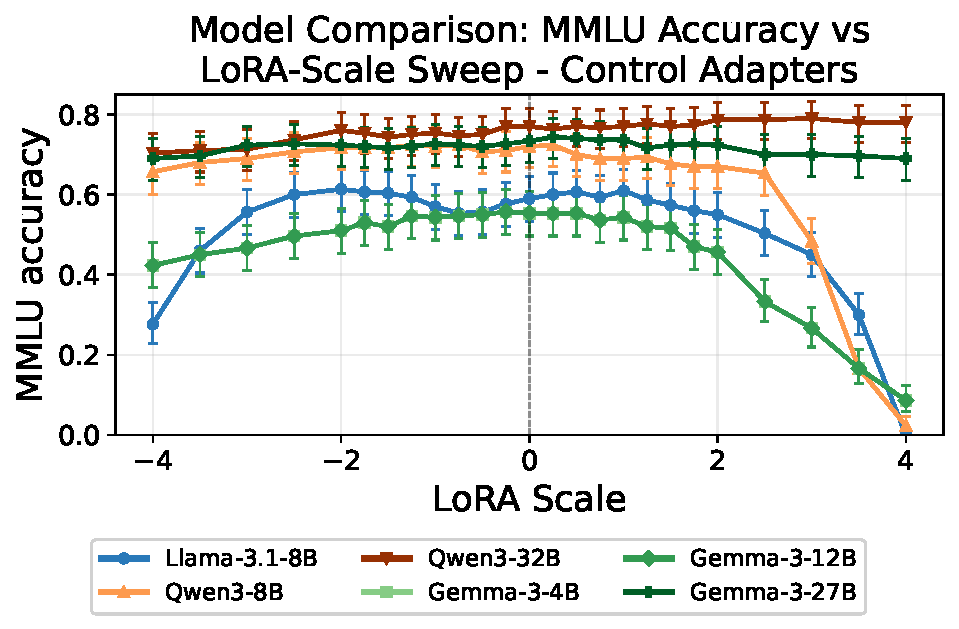
\includegraphics[width=0.6\linewidth]{figures/appendix/model_comparison/fig_crossmodel_mmlu_control.pdf}
\caption{\textbf{Null control adapter MMLU retention across base models.} The
control adapter's MMLU accuracy vs LoRA scale; the capability cost of scaling the
null adapter is the noise floor against which the trait adapters'
\Cref{fig:crossmodel-mmlu} degradation should be read.}
\label{fig:crossmodel-mmlu-control}
\end{figure}

\FloatBarrier
